%!TEX root = ../main.tex
%%%%%%%%%%%%%%%%%%%%%%%%%%%%%%%%%%
% Links:
%
% Difficulty:
% Companies: 
%%%%%%%%%%%%%%%%%%%%%%%%%%%%%%%%%%


%\begin{figure}
%	\centering
%	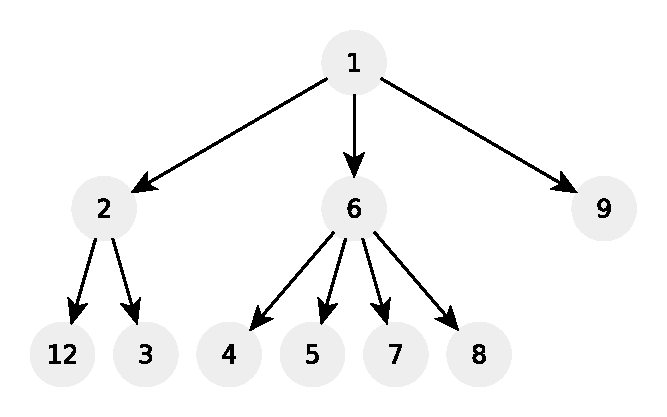
\includegraphics[width=\textwidth]{sources/count_bits/images/example1}
%	\caption[Sample short cpation]{Sample Caption}.
%	\label{fig:count_bits:example1}
%\end{figure}

\chapter{Count the bits}
\label{ch:count_bits}
\section*{Introduction}

\section{Problem statement}
\begin{exercise}
\label{example:count_bits:exercice1}
Given a non negative integer number $n$
return an array $B$ of size $n+1$ where $B_i$ contains the 
number of bits set in the number $i$.
	%example1
	\begin{example}
		\label{example:count_bits:example1}
		\hfill \\
	
		
	\end{example}

	%example2
	\begin{example}
		\label{example:count_bits:example2}
		\hfill \
		
	\end{example}

	\begin{example}
		\hfill \
	
	\label{ex:count_bits:example3}
	\end{example}

	\begin{example}
		\hfill \

	\label{ex:count_bits:example4}	
	\end{example}
\end{exercise}

\section{Clarification Questions}

\begin{QandA}
	\item Can we assume $n$ is always positive?
	\begin{answered}
		\textit{Yes you do not have to do any input validation}
	\end{answered}
	
\end{QandA}

\section{Discussion}
\label{count_bits:sec:discussion}


Thinking:

We do not need check the input parameter, because the question has already mentioned that the number is non negative.

How we do this? The first idea come up with is find the pattern or rules for the result. Therefore, we can get following pattern

Index : 0 1 2 3 4 5 6 7 8 9 10 11 12 13 14 15

num : 0 1 1 2 1 2 2 3 1 2 2 3 2 3 3 4

Do you find the pattern?

Obviously, this is overlap sub problem, and we can come up the DP solution. For now, we need find the function to implement DP.

\subsection{Brute-force}
\label{count_bits:sec:bruteforce}

\begin{minipage}{\linewidth}
	\lstinputlisting[language=c++, caption={Sample Caption},label=list:count_bits]{sources/count_bits/count_bits_solution1.cpp}
\end{minipage}

